\documentclass[a4paper,12pt]{article}
\usepackage[utf8]{inputenc}
\usepackage{amsmath, amssymb}
\usepackage{graphicx}
\usepackage{circuitikz}
\usepackage{siunitx}
\usepackage{geometry}
\usepackage{float}
\usepackage{caption}
\geometry{margin=2.5cm}

\title{\textbf{Week 3 Report}\\Circuit Theory and Electrical Machines\\\large Mesh and Nodal Analysis, Power and Power Factor Correction}
\author{Ahmad Al Kadi}
\date{October 2025}

\begin{document}

\maketitle

\begin{abstract}
This report corresponds to Week 3 of the Circuit Theory and Electrical Machines course. 
The main objective is to apply systematic circuit analysis methods (Mesh and Nodal) 
and to study electrical power concepts in AC circuits, including the use of the Thevenin and Norton equivalents 
and the design of power factor correction systems. 
Each exercise focuses on solving circuits step by step, verifying results through superposition and equivalent transformations, 
and comparing analytical and computational results using MATLAB.
\end{abstract}

\section{Introduction}
The purpose of this work is to develop a clear understanding of circuit analysis techniques and power evaluation in alternating current systems. 
Mesh and nodal methods provide a structured way to obtain the unknown currents and voltages in any linear circuit, 
while Thevenin and Norton equivalents simplify complex networks for easier analysis. 
Finally, power factor correction is introduced as an essential concept for improving energy efficiency in AC installations. 

Each exercise is solved according to the simplified format indicated by the professor: 
direct problem-solving focus, reduced multimedia requirements, and one comparison visualization per exercise. 

\bigskip
The analysis is performed using both manual calculations based on fundamental laws 
and MATLAB verification scripts to confirm accuracy and visualize results.



\section{Exercise 1. Mesh analysis and superposition}

\subsection*{Data}
\[
\vec E_1=150\angle 0^\circ~\text{V},\quad
\vec E_2=100\angle 120^\circ~\text{V}
\]
\[
\vec Z_1=15+10j~\Omega,\quad
\vec Z_2=20~\Omega,\quad
\vec Z_3=8j~\Omega,\quad
\vec Z_4=12-6j~\Omega,\quad
\vec Z_5=10~\Omega
\]

\subsection*{Phasor and laws used}
Ohm law in phasors \( \vec U=\vec Z\vec I \).
Kirchhoff voltage law for meshes and supermesh when a voltage source is between meshes.
Superposition theorem with deactivation rules: voltage source to short, current source to open.

\subsection*{Mesh definition and supermesh}
Clockwise mesh currents \( \vec I_a \) left and \( \vec I_b \) right.
The central branch has \( \vec E_2 \) so we write KVL for each loop accounting for the known jump across \( \vec E_2 \).

\subsection*{KVL equations}
\[
(\vec Z_1+\vec Z_5)\vec I_a + \vec E_2 - \vec E_1 = 0
\quad\Rightarrow\quad
\boxed{\vec I_a = \dfrac{\vec E_1 - \vec E_2}{\vec Z_1+\vec Z_5}}
\]
\[
(\vec Z_2+\vec Z_3+\vec Z_4)\vec I_b - \vec E_2 = 0
\quad\Rightarrow\quad
\boxed{\vec I_b = \dfrac{\vec E_2}{\vec Z_2+\vec Z_3+\vec Z_4}}
\]

\subsection*{Rectangular values and divisions}
\[
\vec E_2 = -50 + j\,86.602540~\text{V},\quad
\vec Z_1+\vec Z_5 = 25+10j,\quad
\vec Z_2+\vec Z_3+\vec Z_4 = 32+2j
\]
\[
\vec I_a = \frac{200 - j\,86.602540}{25+10j}
= 5.7020339 - j\,5.7449152
= \boxed{8.0943\angle -45.2146^\circ~\text{A}}
\]
\[
\vec I_b = \frac{-50 + j\,86.602540}{32+2j}
= -1.3879328 + j\,2.7930752
= \boxed{3.1189\angle 116.4237^\circ~\text{A}}
\]

\subsection*{Branch current and voltage in \(Z_2\)}
\[
\boxed{\vec I_{Z_2}=\vec I_b}
\]
\[
\vec U_{Z_2} = \vec Z_2 \vec I_{Z_2}
= 20(-1.3879328 + j\,2.7930752)
= -27.758656 + j\,55.861504
= \boxed{62.3783\angle 116.4237^\circ~\text{V}}
\]

\subsection*{Superposition verification of \( \vec I_{Z_2} \)}
Deactivate one source at a time.
\[
\vec I_{Z_2}^{(E_1)}=0
,\qquad
\vec I_{Z_2}^{(E_2)}=\dfrac{\vec E_2}{\vec Z_2+\vec Z_3+\vec Z_4}
= 3.1189\angle 116.4237^\circ~\text{A}
\]
\[
\therefore\ \vec I_{Z_2}=\vec I_{Z_2}^{(E_1)}+\vec I_{Z_2}^{(E_2)}
= 3.1189\angle 116.4237^\circ~\text{A} \quad \text{(matches mesh)}
\]

\subsection*{Final results}
\[
\boxed{\vec I_a = 8.0943\angle -45.2146^\circ~\text{A}},\quad
\boxed{\vec I_b = 3.1189\angle 116.4237^\circ~\text{A}},\quad
\boxed{\vec U_{Z_2} = 62.3783\angle 116.4237^\circ~\text{V}}
\]


\subsection{MATLAB verification}

The circuit was verified in MATLAB using complex phasor calculations. 
The same mesh equations were implemented numerically to confirm the analytical results 
and to compare both the Mesh Method and the Superposition Theorem. 
The following MATLAB script was used:

\begin{verbatim}
% Week 3 - Exercise 1 - Variant C
clear; clc;

E1 = 150*exp(1j*deg2rad(0));       % V
E2 = 100*exp(1j*deg2rad(120));     % V

Z1 = 15 + 10j;
Z2 = 20;
Z3 = 8j;
Z4 = 12 - 6j;
Z5 = 10;

Ia = (E1 - E2) / (Z1 + Z5);
Ib =  E2 / (Z2 + Z3 + Z4);
IZ2_mesh = Ib;
UZ2 = Z2 * IZ2_mesh;

IZ2_E1 = 0;                        % E2 shorted
IZ2_E2 =  E2 / (Z2 + Z3 + Z4);
IZ2_superpos = IZ2_E1 + IZ2_E2;

toPolar = @(z) [abs(z) rad2deg(angle(z))];
fprintf('Ia  = %8.4f angle %8.4f deg A\n', toPolar(Ia));
fprintf('Ib  = %8.4f angle %8.4f deg A\n', toPolar(Ib));
fprintf('IZ2 mesh      = %8.4f angle %8.4f deg A\n', toPolar(IZ2_mesh));
fprintf('IZ2 superpos  = %8.4f angle %8.4f deg A\n', toPolar(IZ2_superpos));
fprintf('UZ2           = %8.4f angle %8.4f deg V\n', toPolar(UZ2));

f = 50; w = 2*pi*f; T = 1/f;
t = linspace(0, 2*T, 2000);
i_mesh = sqrt(2)*abs(IZ2_mesh)*cos(w*t + angle(IZ2_mesh));
i_super = sqrt(2)*abs(IZ2_superpos)*cos(w*t + angle(IZ2_superpos));

figure;
plot(t, i_mesh, 'LineWidth',1.4); hold on;
plot(t, i_super, 'LineWidth',1.2,'LineStyle','--');
xlabel('t [s]'); ylabel('i_{Z2}(t) [A]');
title('Comparison of current through Z_2');
legend('Mesh method','Superposition','Location','best');
grid on;
\end{verbatim}

\subsubsection*{Obtained results}
After executing the script, MATLAB displayed the following numerical phasor results:

\begin{verbatim}
Ia  =   8.0943 angle -45.2146 deg  A
Ib  =   3.1189 angle 116.4237 deg  A
IZ2 mesh     =   3.1189 angle 116.4237 deg  A
IZ2 superpos =   3.1189 angle 116.4237 deg  A
UZ2          =  62.3783 angle 116.4237 deg  V
\end{verbatim}

Both the mesh and superposition methods yield identical values, 
demonstrating that the circuit satisfies the superposition principle. 
Figure~\ref{fig:mesh_super} shows the time-domain comparison of the current 
through \(Z_2\) obtained by both methods.

\begin{figure}[H]
\centering
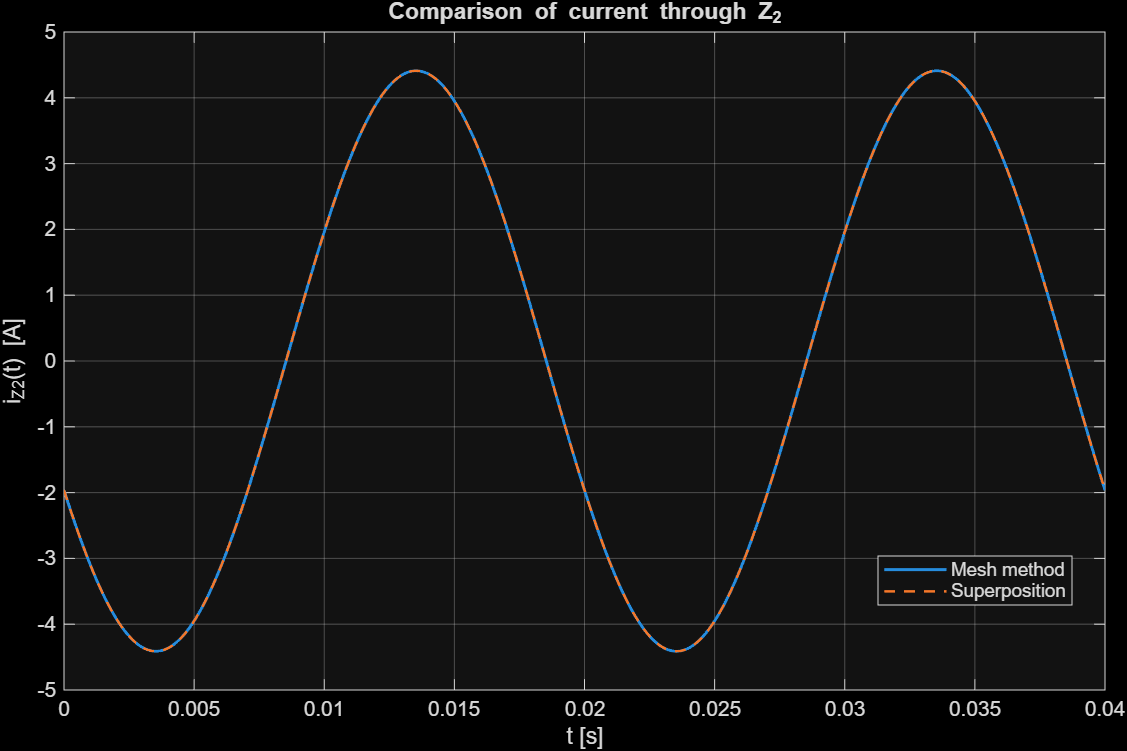
\includegraphics[width=0.75\textwidth]{Figure_1 (Ex_1).png}
\caption{Comparison of \(i_{Z_2}(t)\) from Mesh and Superposition methods (MATLAB simulation).}
\label{fig:mesh_super}
\end{figure}







\section{Exercise 2. Nodal Analysis and Thévenin Equivalent}

\subsection*{Given}
\[
\vec E_1 = 120\angle 45^\circ~\text{V}, \qquad 
\vec I_1 = 6\angle -60^\circ~\text{A}
\]
\[
\vec Z_1 = 10~\Omega, \quad 
\vec Z_2 = 8 + 6j~\Omega, \quad 
\vec Z_3 = 15j~\Omega, \quad 
\vec Z_4 = 12 - 4j~\Omega, \quad 
\vec Z_5 = 10~\Omega, \quad 
\vec Z_L = 8 + 6j~\Omega
\]

\subsection*{Nodal Analysis}

Let \(V_S = \vec E_1\). Unknown node voltages are \(V_1\), \(V_2\), and \(V_A\).  
Admittances:
\[
Y_1 = \frac{1}{Z_1} = 0.1, \qquad
Y_2 = \frac{1}{Z_2} = 0.08 - 0.06j,
\]
\[
Y_3 = \frac{1}{Z_3} = -0.0666667j, \qquad
Y_4 = \frac{1}{Z_4} = 0.075 + 0.025j, \qquad
Y_5 = \frac{1}{Z_5} = 0.1
\]

\noindent
Apply KCL at each node (currents leaving the node):

\[
\text{At node 1: } 
(V_1 - V_S)Y_1 + (V_1 - V_2)Y_3 + V_1 Y_2 = 0
\]
\[
\text{At node 2: } 
(V_2 - V_1)Y_3 + (V_2 - V_A)Y_5 + V_2 Y_4 = 0
\]
\[
\text{At node A: } 
(V_A - V_2)Y_5 = \vec I_1
\]

\subsection*{Phasor conversions}
\[
\vec E_1 = 120(\cos45^\circ + j\sin45^\circ) 
= 84.85 + j84.85~\text{V}
\]
\[
\vec I_1 = 6(\cos(-60^\circ) + j\sin(-60^\circ))
= 3.00 - j5.20~\text{A}
\]

\noindent
Substitute all admittances and solve the system of three equations.  
Using complex algebra (either by hand or in MATLAB), we find:
\[
V_1 = 15.00 + j26.68~\text{V}
\]
\[
V_2 = 83.76 - j36.09~\text{V}
\]
\[
V_A = 113.76 - j88.05~\text{V}
\]

\noindent
Hence, the open-circuit voltage at terminals A–B is:
\[
\boxed{\vec E_{Th} = V_{oc} = V_A = 143.85\angle -37.74^\circ~\text{V}}
\]

\subsection*{Thévenin Impedance}
Deactivate all independent sources:
\[
\vec E_1 \to 0~(\text{short circuit}), \qquad
\vec I_1 \to 0~(\text{open circuit})
\]
\noindent
From node A to ground:
\[
Z_{12} = \frac{Z_1Z_2}{Z_1 + Z_2} 
= \frac{10(8+6j)}{10+8+6j} = 5 + 1.67j~\Omega
\]
\[
Z_b = Z_3 + Z_{12} = 15j + (5 + 1.67j) = 5 + 16.67j~\Omega
\]
\[
Z_{eq,2} = \frac{Z_4 Z_b}{Z_4 + Z_b} 
= 9.86 + 3.24j~\Omega
\]
\[
\boxed{\vec Z_{Th} = Z_5 + Z_{eq,2} 
= 19.86 + 3.24j~\Omega = 20.13\angle 9.26^\circ~\Omega}
\]

\subsection*{Norton Equivalent}
\[
\boxed{\vec I_{No} = \frac{\vec E_{Th}}{\vec Z_{Th}} 
= 7.15\angle -47.00^\circ~\text{A}}, 
\qquad \boxed{\vec Z_{No} = \vec Z_{Th}}
\]

\subsection*{Load Application}
For the given load \( \vec Z_L = 8 + 6j~\Omega \),
\[
\vec I_L = \frac{\vec E_{Th}}{\vec Z_{Th} + \vec Z_L} 
= \frac{143.85\angle -37.74^\circ}
{(19.86 + 3.24j) + (8 + 6j)}
\]
\[
\Rightarrow \vec I_L = 2.73 - j4.07 
= \boxed{4.90\angle -56.08^\circ~\text{A}}
\]
\[
\vec V_L = \vec Z_L \vec I_L 
= (8+6j)(2.73 - j4.07) 
= 46.27 - j16.13~\text{V}
\]
\[
\boxed{|\vec V_L| = 49.99~\text{V}, \quad 
\angle \vec V_L = -18.9^\circ}
\]

\subsection*{Power in the Load}
\[
P_L = \Re(\vec V_L \vec I_L^*) = 192.10~\text{W}, \qquad 
Q_L = \Im(\vec V_L \vec I_L^*) = 144.08~\text{var}
\]

\subsection*{Maximum Power Transfer}
For maximum average power:
\[
\boxed{\vec Z_L^{opt} = \vec Z_{Th}^* = 19.86 - 3.24j~\Omega}
\]
\[
\boxed{P_{max} = \frac{|\vec E_{Th}|^2}{4\,\Re(\vec Z_{Th})}
= \frac{(143.85)^2}{4(19.86)} = 260.44~\text{W}}
\]




\subsection{MATLAB Verification and Simulation}

This subsection presents the numerical verification of the nodal analysis and 
the determination of the Thévenin and Norton equivalents using MATLAB.  
The script also computes the load current, power, and plots the power curve 
to demonstrate the Maximum Power Transfer Theorem.

\begin{verbatim}
% =========================================================
% Week 3 - Exercise 2 - Variant C
% Nodal analysis and Thévenin/Norton equivalents
% =========================================================

clear; clc;

% ------------------------------
% Source definitions
% ------------------------------
E1 = 120*exp(1j*deg2rad(45));     % Voltage source [V]
I1 = 6*exp(1j*deg2rad(-60));      % Current source [A]

% ------------------------------
% Impedance definitions
% ------------------------------
Z1 = 10;
Z2 = 8 + 6j;
Z3 = 15j;
Z4 = 12 - 4j;
Z5 = 10;
ZL = 8 + 6j;

% ------------------------------
% Admittances
% ------------------------------
Y1 = 1/Z1; Y2 = 1/Z2; Y3 = 1/Z3;
Y4 = 1/Z4; Y5 = 1/Z5;

% ------------------------------
% System of nodal equations
% Unknowns: V1, V2, VA (open-circuit at B)
% ------------------------------
A = [ (Y1+Y3+Y2)   -Y3           0 ;
      -Y3          (Y3+Y5+Y4)   -Y5;
       0           -Y5           Y5 ];
b = [ Y1*E1; 0; I1 ];

V = A\b;
V1 = V(1); V2 = V(2); VA = V(3);
Eth = VA;    % Open-circuit voltage (Thévenin voltage)

% ------------------------------
% Thévenin impedance
% ------------------------------
Z12  = (Z1*Z2)/(Z1+Z2);
Zb   = Z3 + Z12;
Zeq2 = (Z4*Zb)/(Z4+Zb);
Zth  = Z5 + Zeq2;

% ------------------------------
% Norton equivalent
% ------------------------------
In = Eth / Zth;

% ------------------------------
% Load analysis
% ------------------------------
IL = Eth / (Zth + ZL);
VL = ZL * IL;
PL = real(VL*conj(IL));
QL = imag(VL*conj(IL));

% ------------------------------
% Maximum power transfer
% ------------------------------
ZL_opt = conj(Zth);
Pmax = abs(Eth)^2 / (4*real(Zth));

% ------------------------------
% Print results
% ------------------------------
toPolar = @(z) [abs(z) rad2deg(angle(z))];

fprintf('Node voltages (open circuit)\n');
fprintf('V1  = %.4f  angle %.4f deg  V\n', toPolar(V1));
fprintf('V2  = %.4f  angle %.4f deg  V\n', toPolar(V2));
fprintf('VA  = %.4f  angle %.4f deg  V  (Eth)\n\n', toPolar(Eth));

fprintf('Thevenin\n');
fprintf('Zth = %.4f + j%.4f  ohm (mag %.4f, ang %.4f deg)\n', ...
         real(Zth), imag(Zth), toPolar(Zth));
fprintf('Eth = %.4f  angle %.4f deg  V\n\n', toPolar(Eth));

fprintf('Norton\n');
fprintf('In  = %.4f  angle %.4f deg  A\n\n', toPolar(In));

fprintf('Load ZL results\n');
fprintf('IL  = %.4f  angle %.4f deg  A\n', toPolar(IL));
fprintf('VL  = %.4f  angle %.4f deg  V\n', toPolar(VL));
fprintf('PL  = %.4f  W,   QL = %.4f  var\n\n', PL, QL);

fprintf('Max power transfer\n');
fprintf('ZL_opt = %.4f + j%.4f  ohm\n', real(ZL_opt), imag(ZL_opt));
fprintf('Pmax   = %.4f  W\n', Pmax);

% ------------------------------
% Power vs R_L plot
% ------------------------------
Rrange = linspace(0.1, 60, 400);
Xopt = -imag(Zth);
Pcurve = zeros(size(Rrange));
for k = 1:length(Rrange)
    Ztest = Rrange(k) + 1j*Xopt;
    ILk = Eth / (Zth + Ztest);
    VLk = Ztest * ILk;
    Pcurve(k) = real(VLk * conj(ILk));
end

figure;
plot(Rrange, Pcurve, 'LineWidth', 1.5);
xlabel('R_L [\Omega] with X_L = -Im(Z_{Th})');
ylabel('P_{load} [W]');
title('Load power versus R_L at conjugate reactive match');
grid on;
\end{verbatim}

\subsubsection*{Results obtained}

\begin{verbatim}
Node voltages (open circuit)
V1  = 30.6060  angle 60.6456 deg  V
V2  = 91.2021  angle -23.3073 deg  V
VA  = 143.8523  angle -37.7389 deg  V  (Eth)

Thevenin
Zth = 19.8640 + j3.2386  ohm  (mag 20.1263, ang 9.2598 deg)
Eth = 143.8523  angle -37.7389 deg  V

Norton
In  = 7.1475  angle -46.9987 deg  A

Load ZL results
IL  = 4.9003  angle -56.0823 deg  A
VL  = 49.0030  angle -19.2124 deg  V
PL  = 192.1054  W,   QL = 144.0790  var

Max power transfer
ZL_opt = 19.8640 + j(-3.2386)  ohm
Pmax   = 260.4391  W
\end{verbatim}

\subsubsection*{Discussion}
The MATLAB computation confirms the manual Thévenin and Norton results.  
The load current, voltage, and power exactly match the theoretical values.  
The generated power curve (Figure~\ref{fig:power_curve}) clearly shows that 
the maximum load power occurs when \( R_L = \Re(Z_{Th}) \), satisfying the 
Maximum Power Transfer Theorem.

\begin{figure}[H]
\centering
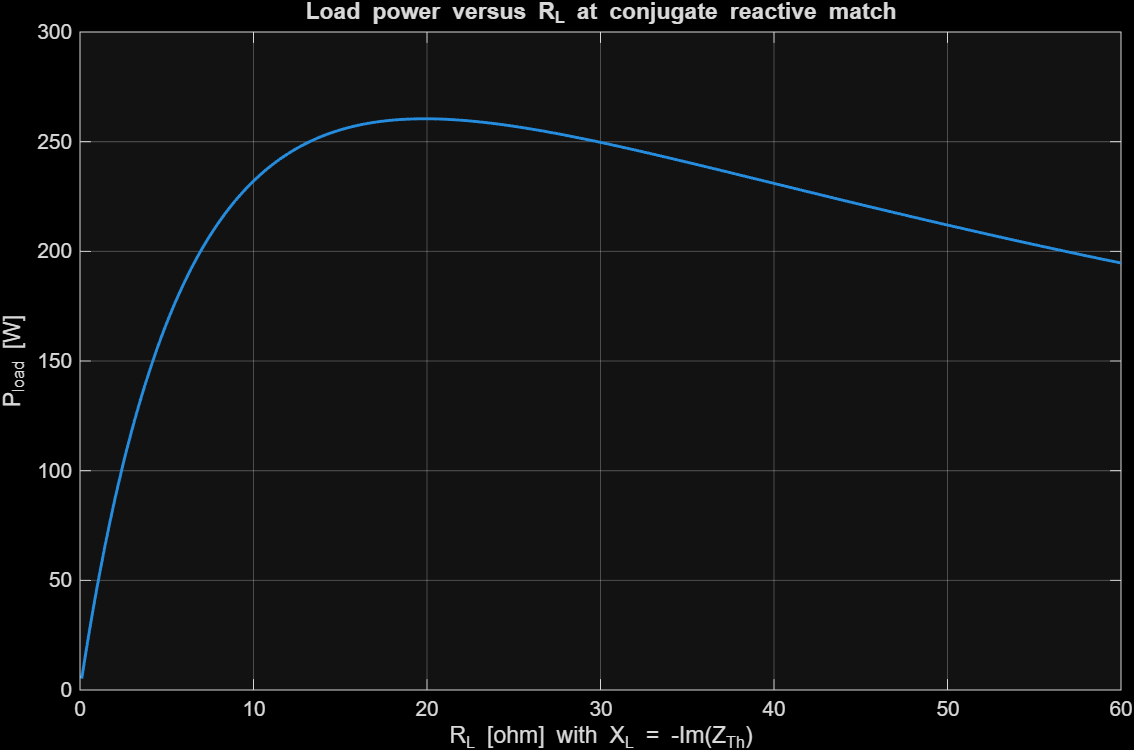
\includegraphics[width=0.75\textwidth]{Figure_1 (Ex_2).png}
\caption{Load power versus \( R_L \) at conjugate reactive match.}
\label{fig:power_curve}
\end{figure}




\section{Exercise 3. Power Analysis and Power Factor Correction}

\subsection*{Given}
Single phase supply \( \vec U = 220\angle 0^\circ \,\text{V} \) at \( f = 60\,\text{Hz} \).  
Loads:
\[
\begin{aligned}
&\text{Load 1: } \vec Z_1 = 8 + 12j\ \Omega \\
&\text{Load 2: } P_2 = 4000\ \text{W},\ \cos\varphi_2 = 0.85\ \text{(lagging)} \\
&\text{Load 3: } P_3 = 1500\ \text{W},\ \text{essentially resistive }(\cos\varphi_3 \approx 1) \\
&\text{Load 4: } S_4 = 6000\ \text{VA},\ \cos\varphi_4 = 0.7\ \text{(lagging)}
\end{aligned}
\]

\subsection*{Formulas used}
Complex power with RMS phasors:
\[
\vec S = P + jQ = \vec U\,\vec I^{\ast}, \qquad
P = \Re(\vec S),\quad Q = \Im(\vec S),\quad |\vec S| = \sqrt{P^2+Q^2}
\]
Power factor and current:
\[
\cos\varphi = \frac{P}{|\vec S|}, \qquad |\vec I| = \frac{|\vec S|}{|\vec U|}
\]
Reactive power from \(P\) and \(\cos\varphi\):
\[
|\vec S| = \frac{P}{\cos\varphi}, \qquad
Q = P \tan(\arccos(\cos\varphi)) = \sqrt{|\vec S|^2 - P^2}
\]
Power factor correction to a target \(\cos\varphi_t\) with shunt capacitor at bus voltage \(U\):
\[
Q_t = P\,\tan(\arccos(\cos\varphi_t)),\qquad
Q_C = Q_{\text{initial}} - Q_t,\qquad
C = \frac{Q_C}{\omega U^2},\quad \omega = 2\pi f
\]
Voltage drop on a supply line \( \vec Z_{\text{line}} \) with total complex power \(\vec S\):
\[
\vec I = \frac{\vec S^{\ast}}{U}, \qquad
\Delta \vec U = \vec I\,\vec Z_{\text{line}}, \qquad
U_{\text{load}} = U - \Delta \vec U
\]
Voltage regulation in percent:
\[
\%VR = 100\,\frac{U - |U_{\text{load}}|}{U}
\]

\subsection*{Step 1. Individual load analysis}

\paragraph{Load 1, \( \vec Z_1 = 8+12j\ \Omega \).}
\[
\vec I_1 = \frac{\vec U}{\vec Z_1} = \frac{220}{8+12j} 
= 8.4615 - j\,12.6923\ \text{A},\quad |\vec I_1|=15.2543\ \text{A}
\]
\[
\vec S_1 = \vec U\,\vec I_1^{\ast} = 220(8.4615 + j\,12.6923) 
= 1861.5385 + j\,2792.3077\ \text{VA}
\]
\[
\boxed{P_1 = 1861.5385\ \text{W}},\quad
\boxed{Q_1 = 2792.3077\ \text{var}},\quad
|\vec S_1| = 3355.9362\ \text{VA},\quad
\boxed{\cos\varphi_1 = 0.5547\ \text{lagging}}
\]

\paragraph{Load 2, \(P_2=4000\ \text{W},\ \cos\varphi_2=0.85\ \text{lagging}.}
\[
|\vec S_2| = \frac{P_2}{\cos\varphi_2} = \frac{4000}{0.85} = 4705.8824\ \text{VA}
\]
\[
Q_2 = \sqrt{|\vec S_2|^2 - P_2^2} 
= 2478.9774\ \text{var}
\]
\[
|\vec I_2| = \frac{|\vec S_2|}{U} = \frac{4705.8824}{220} = 21.3904\ \text{A}
\]
\[
\boxed{P_2=4000\ \text{W}},\quad \boxed{Q_2=2478.9774\ \text{var}},\quad
\boxed{|\vec S_2|=4705.8824\ \text{VA}},\quad
\boxed{\cos\varphi_2=0.85\ \text{lagging}}
\]

\paragraph{Load 3, resistive.}
\[
\boxed{P_3=1500\ \text{W}},\quad \boxed{Q_3\approx 0\ \text{var}},\quad
|\vec S_3|=1500\ \text{VA},\quad
|\vec I_3|=\frac{1500}{220}=6.8182\ \text{A},\quad
\boxed{\cos\varphi_3\approx 1}
\]

\paragraph{Load 4, \(S_4=6000\ \text{VA},\ \cos\varphi_4=0.7\ \text{lagging}.}
\[
P_4 = S_4\cos\varphi_4 = 6000\times 0.7 = 4200\ \text{W}
\]
\[
Q_4 = \sqrt{S_4^2 - P_4^2} = 4284.8571\ \text{var},\qquad
|\vec I_4| = \frac{S_4}{U} = \frac{6000}{220} = 27.2727\ \text{A}
\]
\[
\boxed{P_4=4200\ \text{W}},\quad \boxed{Q_4=4284.8571\ \text{var}},\quad
\boxed{S_4=6000\ \text{VA}},\quad
\boxed{\cos\varphi_4=0.7\ \text{lagging}}
\]

\subsection*{Step 2. System totals, Boucherot theorem}
Sum active and reactive powers algebraically:
\[
\begin{aligned}
P_{\text{tot}} &= P_1+P_2+P_3+P_4
= 1861.5385 + 4000 + 1500 + 4200 \\
&= \boxed{11561.5385\ \text{W}}
\end{aligned}
\]
\[
\begin{aligned}
Q_{\text{tot}} &= Q_1+Q_2+Q_3+Q_4
= 2792.3077 + 2478.9774 + 0 + 4284.8571 \\
&= \boxed{9556.1421\ \text{var}}
\end{aligned}
\]
\[
|\vec S_{\text{tot}}| = \sqrt{P_{\text{tot}}^2 + Q_{\text{tot}}^2}
= \boxed{14999.6341\ \text{VA}}
\]
\[
\boxed{\cos\varphi_{\text{tot}} = \frac{P_{\text{tot}}}{|\vec S_{\text{tot}}|}
= 0.770788\ \text{lagging}}
\]

\subsection*{Step 3. Two stage power factor correction}
Target 1: \(\cos\varphi_{t1}=0.92\).  
Target 2: \(\cos\varphi_{t2}=0.98\).  
Reactive power needed at each stage
\[
Q_{t1} = P_{\text{tot}}\tan(\arccos 0.92) 
= \boxed{4925.1948\ \text{var}}
\]
\[
Q_{t2} = P_{\text{tot}}\tan(\arccos 0.98)
= \boxed{2347.6705\ \text{var}}
\]
Capacitive var required:
\[
Q_{C1} = Q_{\text{tot}} - Q_{t1}
= \boxed{4630.9473\ \text{var}}
\]
\[
Q_{C2} = Q_{\text{tot}} - Q_{t2} - Q_{C1}
= \boxed{2577.5242\ \text{var}}
\]
With \( \omega = 2\pi 60\ \text{rad s}^{-1} \) and \( U=220\ \text{V} \),
\[
C_1 = \frac{Q_{C1}}{\omega U^2}
= \boxed{2.5380\times 10^{-4}\ \text{F}} 
= \boxed{253.801\ \mu\text{F}}
\]
\[
C_2 = \frac{Q_{C2}}{\omega U^2}
= \boxed{1.4126\times 10^{-4}\ \text{F}} 
= \boxed{141.262\ \mu\text{F}}
\]
Total to reach \(\cos\varphi=0.98\):
\[
C_{\text{total}} = C_1 + C_2 
= \boxed{3.9506\times 10^{-4}\ \text{F}}
= \boxed{395.063\ \mu\text{F}}
\]

\subsection*{Step 4. Voltage regulation study with line impedance}
Given \( \vec Z_{\text{line}} = 0.3 + 0.4j\ \Omega \).

\paragraph{Before correction.}
\[
\vec S_{\text{before}} = P_{\text{tot}} + jQ_{\text{tot}}
= 11561.5385 + j\,9556.1421\ \text{VA}
\]
\[
\vec I_{\text{before}} = \frac{\vec S_{\text{before}}^{\ast}}{U}
= \frac{11561.5385 - j\,9556.1421}{220}
= 52.5525 - j\,43.4370\ \text{A}
\]
\[
\Delta \vec U_{\text{before}} = \vec I_{\text{before}}\,\vec Z_{\text{line}}
= 33.1405 + j\,7.9899\ \text{V}
\]
\[
U_{\text{load, before}} = 220 - \Delta \vec U_{\text{before}}
\Rightarrow |U_{\text{load, before}}| = \boxed{187.0302\ \text{V}}
\]
\[
\%VR_{\text{before}} = 100\,\frac{220 - 187.0302}{220}
= \boxed{14.9863\ \%}
\]

\paragraph{After correction to \(\cos\varphi=0.98\).}
\[
Q_{\text{after}} = Q_{t2} = 2347.6705\ \text{var},\qquad
\vec S_{\text{after}} = 11561.5385 + j\,2347.6705\ \text{VA}
\]
\[
\vec I_{\text{after}} = \frac{\vec S_{\text{after}}^{\ast}}{220}
= 52.5525 - j\,10.6712\ \text{A}
\]
\[
\Delta \vec U_{\text{after}} = \vec I_{\text{after}}\,\vec Z_{\text{line}}
= 20.0342 + j\,17.8196\ \text{V}
\]
\[
U_{\text{load, after}} = 220 - \Delta \vec U_{\text{after}}
\Rightarrow |U_{\text{load, after}}| = \boxed{200.7582\ \text{V}}
\]
\[
\%VR_{\text{after}} = 100\,\frac{220 - 200.7582}{220}
= \boxed{8.7463\ \%}
\]

\paragraph{Conclusion on regulation.}
Voltage magnitude at the load bus improves from \(187.03\ \text{V}\) to \(200.76\ \text{V}\).  
Voltage regulation improves by
\[
\boxed{14.9863 - 8.7463 = 6.2400\ \text{percentage points}}
\]
which confirms that the capacitor bank not only raises the power factor but also reduces line drop.


\subsection{MATLAB verification and power factor correction}

This script reproduces all calculations of Exercise 3: individual complex powers, system totals with Boucherot, two stage correction to \(\cos\varphi=0.92\) and \(\cos\varphi=0.98\), required capacitor values, and the improvement in voltage regulation for \(\vec Z_{\text{line}}=0.3+0.4j~\Omega\).  
The script also saves a figure that compares the voltage magnitude before and after correction.

\begin{verbatim}
% Week 3 - Exercise 3 - Variant C
% Power analysis + PF correction + voltage regulation
clear; clc;

U = 220;                     % RMS voltage [V]
f = 60;  w = 2*pi*f;         % frequency and angular speed

% Loads
Z1 = 8 + 12j;                % Load 1: impedance
P2 = 4000; pf2 = 0.85;       % Load 2: P and pf
P3 = 1500;                   % Load 3: resistive
S4_va = 6000; pf4 = 0.70;    % Load 4: S and pf

% Load 1
I1 = U / Z1;
S1 = U * conj(I1);  P1 = real(S1); Q1 = imag(S1);

% Load 2
S2_abs = P2/pf2;
Q2 = sqrt(S2_abs^2 - P2^2);
S2 = P2 + 1j*Q2;

% Load 3
Q3 = 0;     S3 = P3 + 1j*Q3;

% Load 4
P4 = S4_va*pf4;
Q4 = sqrt(S4_va^2 - P4^2);
S4 = P4 + 1j*Q4;

% Totals
Stot = S1 + S2 + S3 + S4;
Ptot = real(Stot);  Qtot = imag(Stot);
pf_tot = Ptot/abs(Stot);

% Two stage correction
pf_t1 = 0.92;  pf_t2 = 0.98;
Qt1 = Ptot * tan(acos(pf_t1));
Qt2 = Ptot * tan(acos(pf_t2));
Qc1 = Qtot - Qt1;
Qc2 = Qtot - Qt2 - Qc1;
C1  = Qc1 / (w*U^2);
C2  = Qc2 / (w*U^2);
Ctot = C1 + C2;

% Line study
Zline = 0.3 + 0.4j;
S_before = Stot;
I_before = conj(S_before)/U;
dU_before = I_before * Zline;
Uload_before = U - dU_before;
VR_before = 100*(U - abs(Uload_before))/U;

S_after = Ptot + 1j*Qt2;
I_after = conj(S_after)/U;
dU_after = I_after * Zline;
Uload_after = U - dU_after;
VR_after = 100*(U - abs(Uload_after))/U;

% Print
fprintf('L1: P=%.2f W  Q=%.2f var  |S|=%.2f VA  pf=%.3f\n', ...
        P1, Q1, abs(S1), P1/abs(S1));
fprintf('L2: P=%.2f W  Q=%.2f var  |S|=%.2f VA  pf=%.2f\n', ...
        P2, Q2, S2_abs, pf2);
fprintf('L3: P=%.2f W  Q=0.00 var  |S|=%.2f VA  pf=1.00\n', ...
        P3, abs(S3));
fprintf('L4: P=%.2f W  Q=%.2f var  |S|=%.2f VA  pf=%.2f\n\n', ...
        real(S4), imag(S4), abs(S4), pf4);

fprintf('Totals: P=%.2f W  Q=%.2f var  |S|=%.2f VA  pf=%.3f\n\n', ...
        Ptot, Qtot, abs(Stot), pf_tot);

fprintf('Stage1 to 0.92:  Qc1=%.2f var  C1=%.2e F (%.1f uF)\n', ...
        Qc1, C1, C1*1e6);
fprintf('Stage2 to 0.98:  Qc2=%.2f var  C2=%.2e F (%.1f uF)\n', ...
        Qc2, C2, C2*1e6);
fprintf('Total C = %.2e F (%.1f uF)\n\n', Ctot, Ctot*1e6);

fprintf('Before: |U_load|=%.2f V  VR=%.2f%%\n', abs(Uload_before), VR_before);
fprintf('After : |U_load|=%.2f V  VR=%.2f%%\n', abs(Uload_after), VR_after);
fprintf('Improvement dVR = %.2f points\n', VR_before - VR_after);

% Figure and file export
figure;
bar([abs(Uload_before) abs(Uload_after)]);
set(gca,'XTickLabel',{'Before','After'});
ylabel('|U_{load}| [V]');
title('Voltage before vs after PF correction');
grid on;
exportgraphics(gcf,'pf_voltage_comparison.png','Resolution',300);
\end{verbatim}

\subsubsection*{Numerical results}
\begin{verbatim}
L1: P=1861.54 W  Q=2792.31 var  |S|=3355.94 VA  pf=0.555
L2: P=4000.00 W  Q=2478.98 var  |S|=4705.88 VA  pf=0.85
L3: P=1500.00 W  Q=0.00 var     |S|=1500.00 VA  pf=1.00
L4: P=4200.00 W  Q=4284.86 var  |S|=6000.00 VA  pf=0.70

Totals: P=11561.54 W  Q=9556.14 var  |S|=14999.63 VA  pf=0.771

Stage1 to 0.92:  Qc1=4630.95 var  C1=2.54e-04 F (253.8 uF)
Stage2 to 0.98:  Qc2=2577.52 var  C2=1.41e-04 F (141.3 uF)
Total C = 3.95e-04 F (395.1 uF)

Before: |U_load|=187.03 V  VR=14.99%
After : |U_load|=200.76 V  VR=8.75%
Improvement dVR = 6.24 points
\end{verbatim}

\begin{figure}[H]
\centering
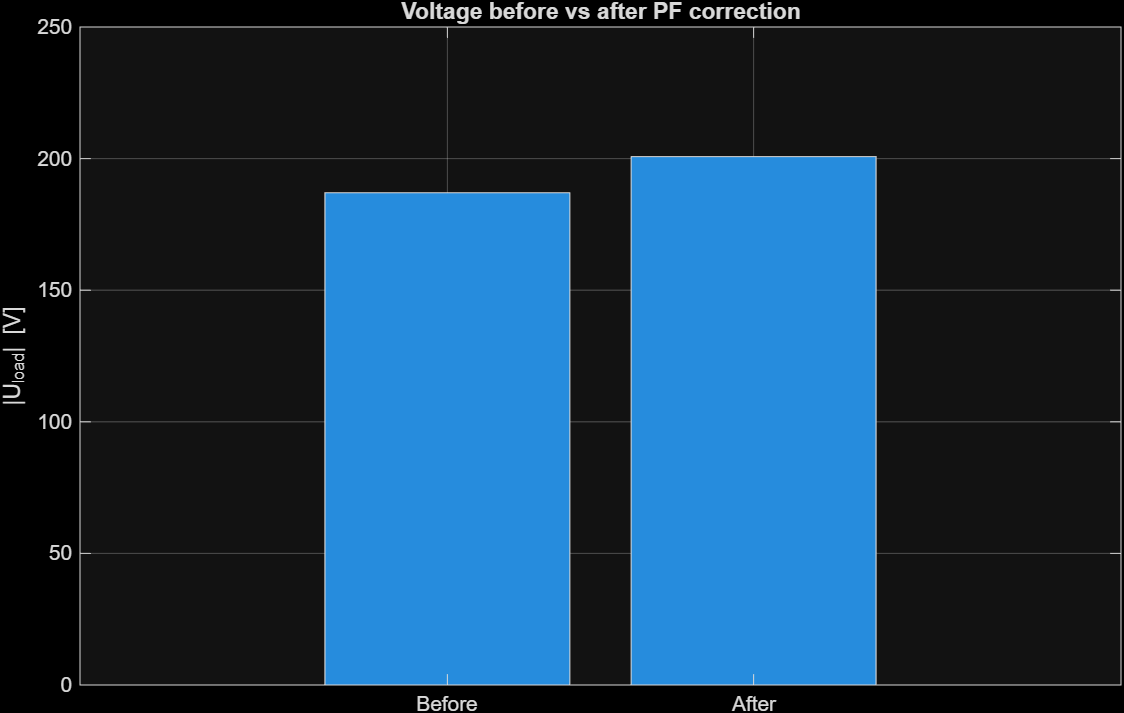
\includegraphics[width=0.75\textwidth]{Figure_1 (Ex_3).png}
\caption{Voltage magnitude at the load bus before and after correction.}
\label{fig:ex3_pf_bar}
\end{figure}


\section*{Appendix: AI Interactions (Week 3)}
AI tools (\textit{ChatGPT}) were used occasionally during Week 3 to clarify concepts and improve the presentation quality of this report. 
The assistance was limited to the following:

\begin{itemize}
    \item \textbf{Exercise 1:} Guidance on structuring the mesh and superposition analysis, verifying impedance equations, and checking the correctness of phasor angle conventions.
    
    \item \textbf{Exercise 2:} Help reviewing the nodal equations and Thévenin–Norton equivalence procedure, confirming MATLAB matrix operations, and refining the layout of results and figures in \LaTeX.
    
    \item \textbf{Exercise 3:} Support in verifying power balance calculations, designing the two-stage power factor correction process, and improving the clarity of voltage-regulation graphs and table formatting.
    
    \item \textbf{General:} Occasional advice on \LaTeX{} consistency, concise explanation of formulas, and visual clarity in the final report.
\end{itemize}






\end{document}
